\documentclass{beamer}

\mode<presentation> 
{
    \usetheme{Madrid}
}

\usepackage[utf8x]{inputenc}
\usepackage[english,russian]{babel}
\usepackage[T2A]{fontenc}
\usepackage{graphicx}
\usepackage{booktabs} 
\usepackage{mathtools}
\usepackage{amsmath}
\usepackage{wasysym}
\usepackage{subfig}
\usepackage{hyperref}
\usepackage{ulem}
\usepackage{ragged2e}
\usepackage{algorithm2e}


\usefonttheme[onlymath]{serif}

\hypersetup
{
    colorlinks=true,
    linkcolor=white, 
    urlcolor=cyan
}

\title[Лекция 1]
{
    Темы для исследовательских работ 
} 


\author[Д. А. Караваев]{Д. А. Караваев}

\institute[СПбГУТ] 
{
    Санкт-Петербургский государственный университет телекоммуникаций \\ им. проф. М. А. Бонч-Бруевича \\ 
    \vspace{0.2cm}
    Факультет РТС, Кафедра РОС \\
    \vspace{0.2cm}
    Факультатив <<Программирование в ЦОС>> \\
    \vspace{0.2cm}
    Осень 2019
}

\date[2019]{Санкт-Петербург} 

\begin{document}
    \begin{frame}
        \titlepage 
    \end{frame}
    \begin{frame}
        \frametitle{Функция (тело) неопределенности на TMS320C6678}
        \begin{equation}
            A[m, \omega_{d}] = \sum_{n=-\infty}^{+\infty}s[n + m] s^{*}[n]e^{j2\pi\omega_{d}(n + m)}
        \end{equation}
        \begin{figure}[!tbp]
           \centering
           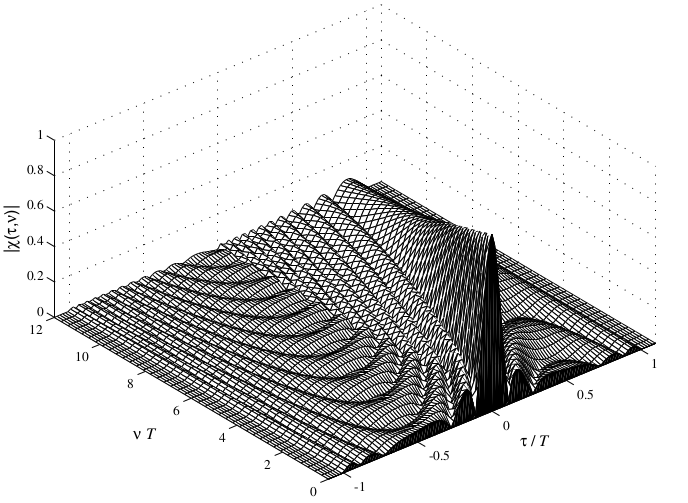
\includegraphics[width=0.5\textwidth]{pics/AF_LFM.png}
           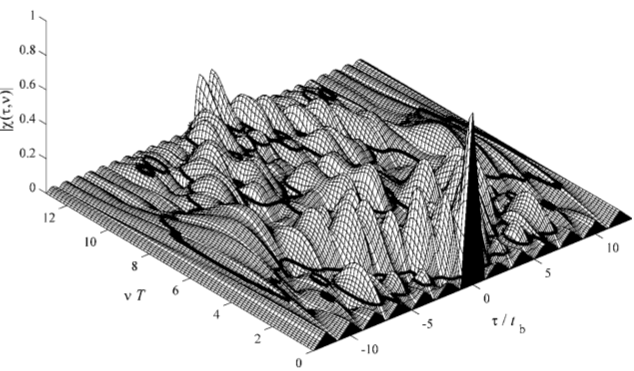
\includegraphics[width=0.5\textwidth]{pics/AF_Barker.png}
           \captionsetup{justification=centering}
           \captionof{figure}{Пример ФН для ЛЧМ сигнала и фазового кода Баркера}
       \end{figure}
    \end{frame}
    \begin{frame}
        \frametitle{Банк фильтров на основе БПФ на TMS320C6678}
        \begin{figure}[!tbp]
           \centering
           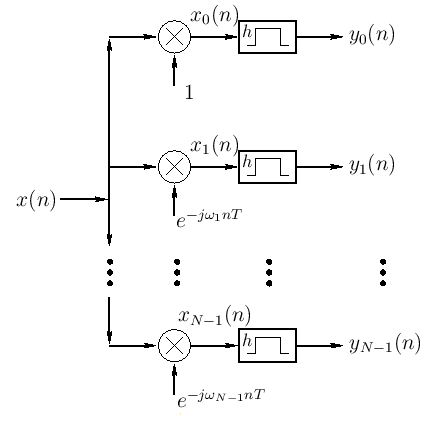
\includegraphics[width=0.4\textwidth]{pics/FB.png}
           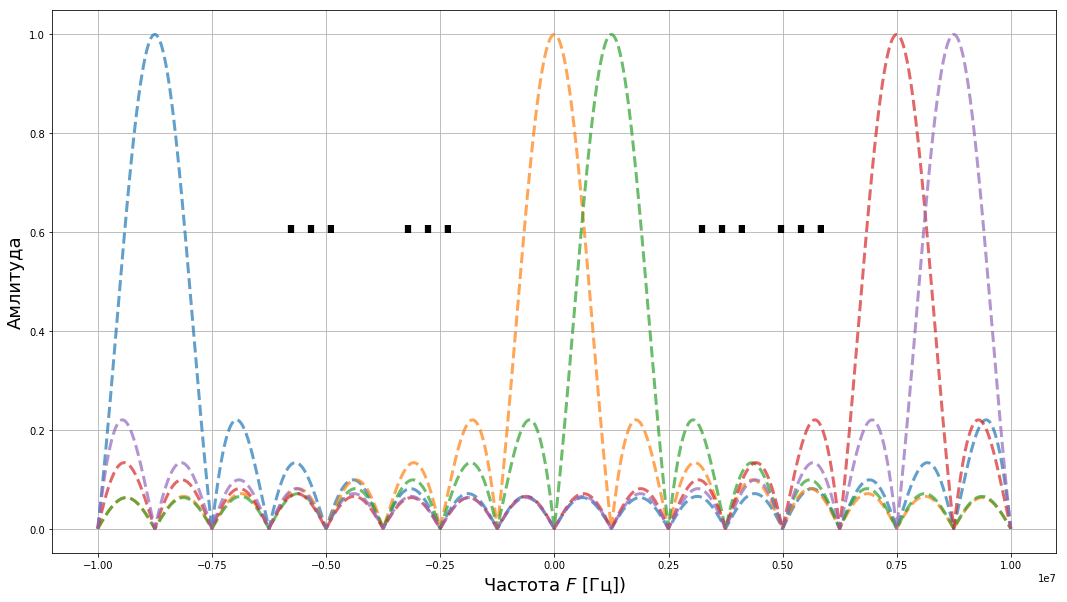
\includegraphics[height=0.55\paperheight, width=0.6\textwidth]{pics/band.png}
           \captionsetup{justification=centering}
           \captionof{figure}{Системная диаграмма банка фильтров и разбинение полосы}
       \end{figure}
    \end{frame}
    \begin{frame}
        \frametitle{Адаптивный фильтр Fast Block LMS на TMS320C6678}
        \begin{figure}[!tbp]
           \centering
           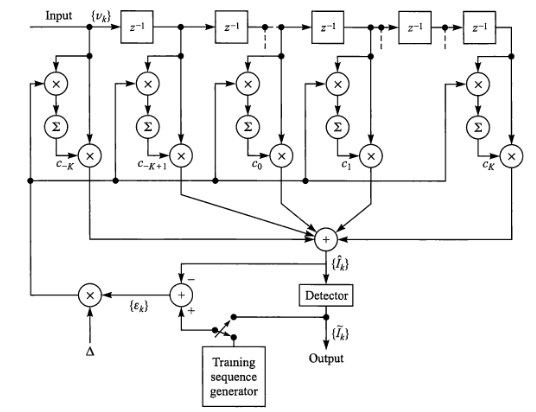
\includegraphics[width=0.75\textwidth]{pics/NLMS.png}
           \captionsetup{justification=centering}
           \captionof{figure}{Пример системной диаграммы адаптивного фильтра}
       \end{figure}
    \end{frame}
    \begin{frame}
        \begin{center}
        \baselineskip 20.0mm
        \Huge Спасибо за внимание!
        \end{center}
    \end{frame}
\end{document}